% -*- coding: utf-8 -*-
\documentclass{beamer}
\usepackage{local}

\usepackage{graphiques}

\mode<handout>{
\usepackage{pgfpages}
\pgfpagesuselayout{2 on 1}[a4paper,border shrink=5mm]}

\title[OtFMI]{\otfmi, an \openturns{} module for~uncertainties~analysis with~\odid~system~models}

\author[Baudin et al.]{
Michaël Baudin \inst{1} \and
Audrey Jardin \inst{1} \and
Mathias Bouquerel \inst{1} \and
Anne-Laure Popelin \inst{1} \and
Audrey Jardin \inst{1} \and
\newline
Julien~Schueller \inst{2} \and
Sylvain~Girard \inst{2}
}\institute[EDF \& Phimeca]{
\inst{1} EDF R\&D. 6, quai Watier, 78401,
Chatou Cedex - France, \url{michael.baudin@edf.fr}
\inst{2} Phimeca Engineering. 18/20 boulevard de Reuilly,
75012 Paris - France, \url{girard@phimeca.com}
}\date[]{October 19th 2017}

\begin{document}
\begin{frame}
\titlepage
\end{frame}

\section{Context}
\label{sec:context}

% ====
\begin{frame}{Industrial issue}
\begin{itemize}
\item \edf{} uses \alert{\odid{} system models} programmed in \alert{\lmodelica{}} as decision support for the conception and operation of its industrial assets.
  % \begin{itemize}
  % \item \edf{} models are programmed in \alert{\lmodelica{}}
  % \end{itemize}
\vfill
\item How to apply \alert{\openturns{}'} panoply of methods to these models?
\end{itemize}
\end{frame}

\begin{frame}[fragile, label=comparaison]{“Regular” models \textit{vs} \odid{} system models}
\tikzexternaldisable{}

\makebox[\textwidth][c]{\centering
  \begin{tikzpicture}
    \tikzset{v composant/.style={visible on=<1-2>},
      vv systeme/.style={visible on=<2>},
      v systeme/.style={visible on=<2->},
      v comparaison/.style={visible on=<3->},
%
      equation composant/.style={cellule, align=center, anchor=north, font=\small,
        fill=white, v composant},
%
      carac etiquette/.style={etiquette, below=1.5em, v comparaison},
      carac composant/.style={align=left, , v comparaison, font cellule},
      carac systeme/.style={align=left, v comparaison, font cellule},
};


\node[cellule] (systeme) at (0,0) {
\includegraphics[height=1.3cm]{./figure/npp}};

\node[cellule, below right=3mm and 5mm, vv systeme] (decoupage) at (systeme.south east) {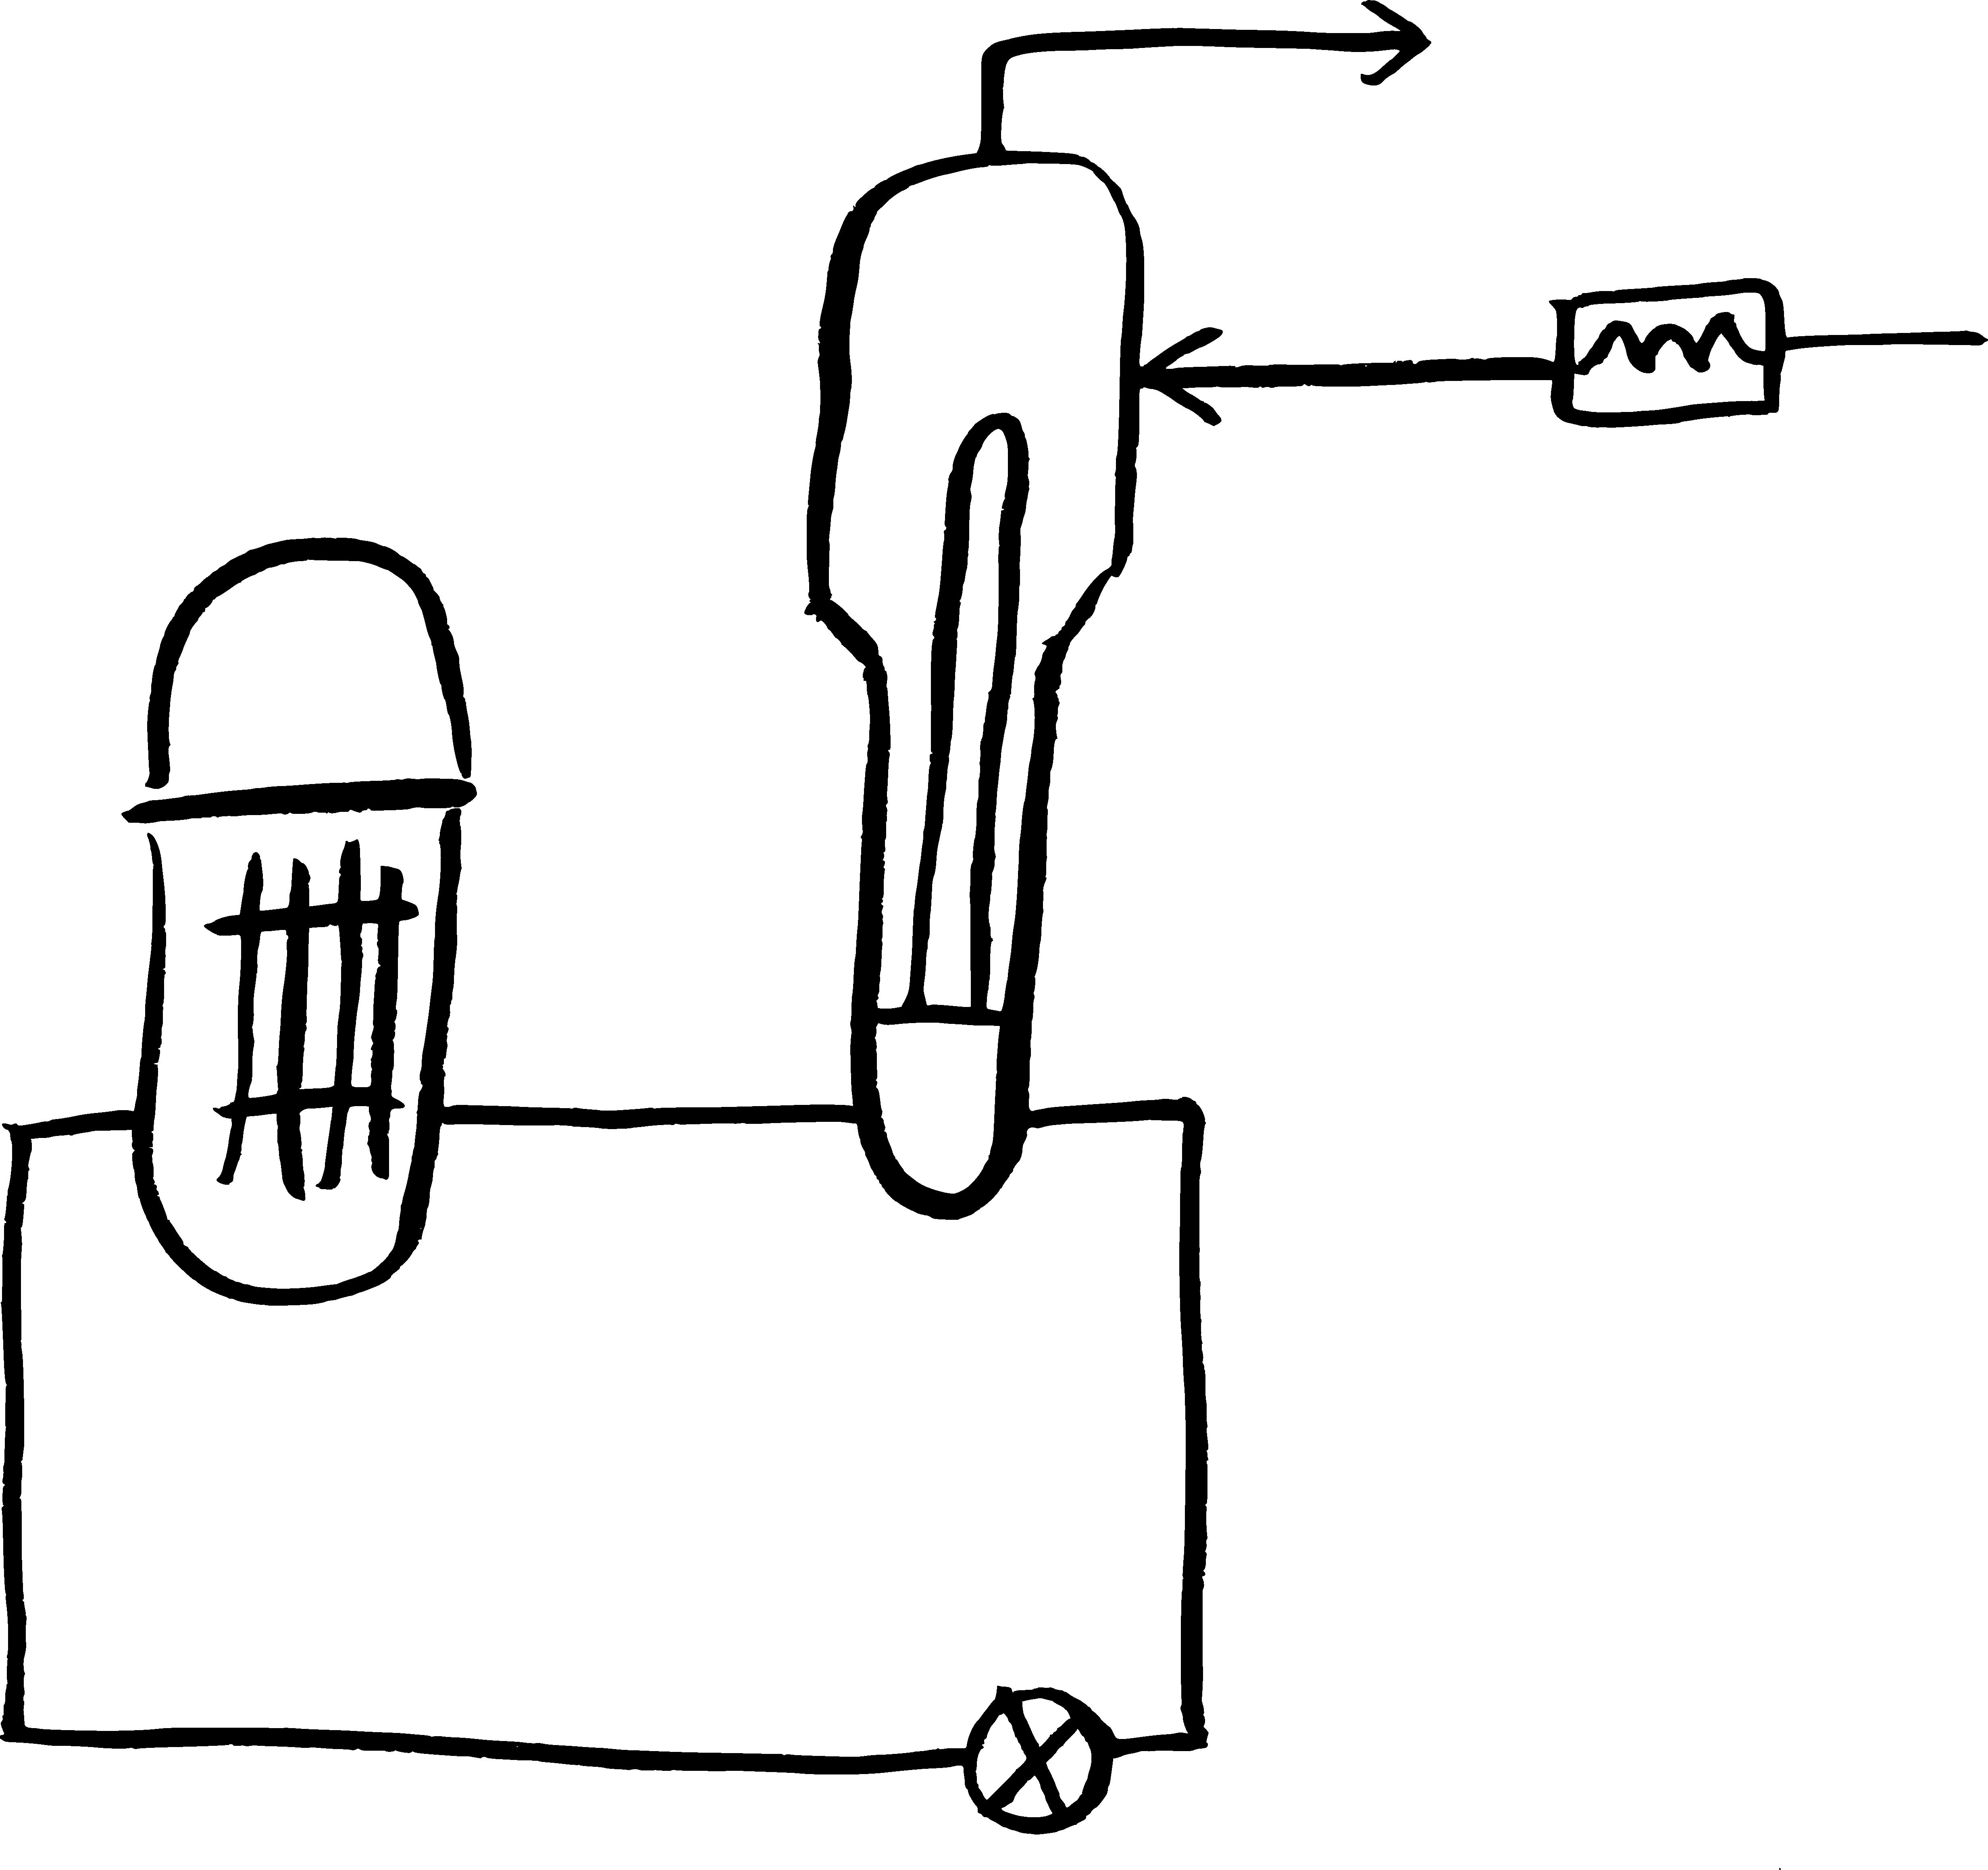
\includegraphics[height=2.2cm]{./figure/decoupage_c}};


\node[cellule, v composant, below left=3mm and 5mm] (gv) at (systeme.south west) {
\includegraphics[height=2.2cm]{./figure/gv}};
\node[cellule, v composant, left=1mm] (cuve) at (gv.west) {
\includegraphics[height=2.2cm]{./figure/cuve}};
\node[cellule, v composant, left=1mm] (pompe) at (cuve.west) {
\includegraphics[height=.5cm]{./figure/pompe}};

\node[cellule, below=3mm, align=center, font=\small, vv systeme] (equation) at (decoupage.south) {\systemeequation};

\node[equation composant, xshift=13mm] (equation pompe) at (pompe.south |- equation.north) {\systemeequation};
\node[equation composant, right=2mm] (equation cuve) at (equation pompe.west) {\systemeequation};
\node[equation composant, right=2mm] (equation gv) at (equation cuve.west) {\systemeequation};

\coordinate[yshift=-12mm] (code) at (equation.south);
\pic[file style, "Modelica", vv systeme, xshift=12mm]  at (code) {file icon};
\pic[file style, "Symulink", vv systeme, xshift=-12mm]  at (code) {file icon};

\pic[file style, "C++", v composant] at (pompe |- code) {file icon};
\pic[file style, "Éléments finis", xshift=4mm, v composant] at (cuve |- code) {file icon};
\pic[file style, "CFD", xshift=6mm, v composant] at (gv |- code) {file icon};


\node[etiquette, above=1mm, xshift=-2mm] at (systeme.east) {Real system};

\node[etiquette, v composant] (etiquette decoupage) at (systeme |- decoupage) {“Packing”};
\node[etiquette, v composant] (etiquette equation) at (systeme |- equation) {Equation formulation};
\node[etiquette, v composant, align=center] at (systeme |- code) {Solver\\programming};

% En-tête
\node[cellule,  align=center, draw=none, v systeme] (titre systeme) at (systeme -| decoupage) {0D/1D\\system modelling};
\node[cellule, align=center, draw=none] (titre composant) at (systeme -| cuve) {“Regular”\\modelling};

% Séparation réel-modèle
\draw[thick, dashed, gray] ([yshift=-1.5mm]systeme.south west -| equation pompe.west)--([yshift=-1.5mm]systeme.south west -| equation.east);

% ================
\coordinate (tmp) at (systeme.south);

\node[carac etiquette] (tmp) at (tmp.south) {CPU time};
\node[carac composant] at (tmp -| titre composant) {Long (minute $\rightarrow$ hour)};
\node[carac systeme] at (tmp -| titre systeme) {Short (second $\rightarrow$ minute)};



\node[carac etiquette] (tmp) at (tmp.south) {Dimensions};
\node[carac composant] at (tmp -| titre composant) {2D, 3D};
\node[carac systeme] at (tmp -| titre systeme) {0D, 1D};

\node[carac etiquette] (tmp) at (tmp.south) {Development rate};
\node[carac composant] at (tmp -| titre composant) {Discrete versioning};
\node[carac systeme] at (tmp -| titre systeme) {Continuous mutation};

\node[carac etiquette] (tmp) at (tmp.south) {Actors};
\node[carac composant] at (tmp -| titre composant) {Numerical analyst, physicist};
\node[carac systeme] at (tmp -| titre systeme) {Design, process, operation\ldots\\engineer};

% \node[carac etiquette] (tmp) at (tmp.south) {Équations de fermeture};
% \node[carac composant] at (tmp -| titre composant) {Phénoménologiques};
% \node[carac systeme] at (tmp -| titre systeme) {Empiriques};


\node[carac etiquette] (tmp) at (tmp.south) {Tools};
\node[carac composant] at (tmp -| titre composant) {CFD, finite elements,\\C++, FORTRAN\ldots};
\node[carac systeme] at (tmp -| titre systeme) {Modelica, Simulink\ldots};

  \end{tikzpicture}

}
\end{frame}

\begin{frame}{\lmodelica{} programming language}
  \begin{itemize}
  \item \lmodelica{} is an open language for programming models based on \alert{differential algebraic systems of equations}
    \vfill
    \makebox[0.9\textwidth][c]{\centering%

\includegraphics[height=1.5cm]{./figure/logo_modelica}}
  \item Equations are written in almost \alert{natural language}, and solved by a multipurpose third party tool.
    \vfill
  \item It is object-oriented: available \alert{module libraries} cover most applications
    \begin{itemize}
    \item Complex models can be achieved simply by combining this modules using a graphical interface!
    \end{itemize}
  \end{itemize}
\end{frame}

\begin{frame}{\lmodelica{} tools}
  \begin{itemize}
  \item Main tools :
    \begin{itemize}
    \item Dymola (Dassault Systèmes, proprietary)
    \item \openmodelica{} (Open Source Modelica Consortium, open source)
  \end{itemize}
\vfill
  \item Functions
    \begin{itemize}
    \item Flatten equation systems
    \item Compile to machine code after including a solver
    \item Development environment
    \item Model graphical interface
    \item Basic post-processing\ldots
    \end{itemize}
  \end{itemize}
\end{frame}

\begin{frame}{\openmodelica{}, model graphical view}
\makebox[\textwidth][c]{\centering%
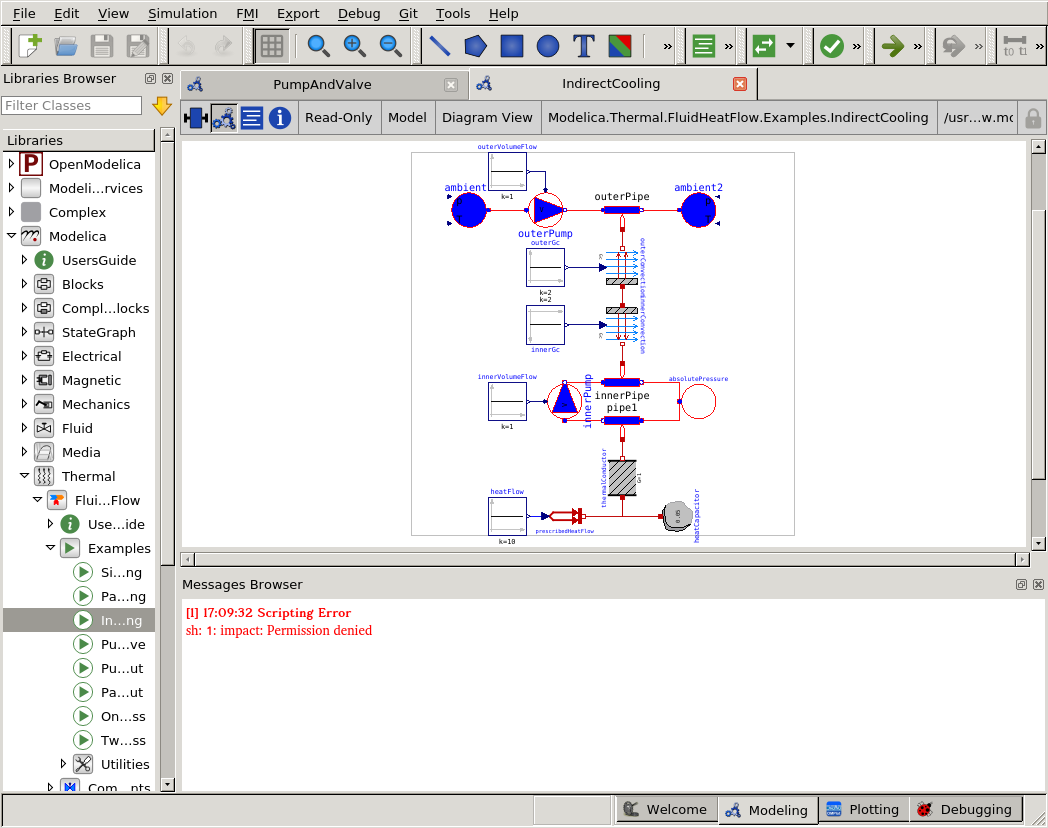
\includegraphics[height=.86\textheight]{./figure/open_modelica_screenshot}
}\end{frame}

\newcommand{\inout}[3]{%
  \foreach \x in {0,1,...,#2} \coordinate (#1 in \x) at ($\x/#2 *(#1.south west) +  1 - \x/#2 *(#1.north west)$);
  \foreach \y in {0,1,...,#3} \coordinate (#1 out \y) at ($\y/#3 *(#1.south east) +  1 - \y/#3 *(#1.north east)$);
}\newcommand{\inmod}[4][1cm]{\draw[link, reverse] (#2 in #3)--++(-#1, 0) node[pos=.5, above] {#4};}
\newcommand{\outmod}[4][1cm]{\draw[link] (#2 out #3)--++(#1, 0) node[pos=.5, above] {#4};}

\begin{frame}{Piloting models}
  \tikzexternaldisable{}
  \begin{itemize}
  \item Most \openturns{} methods apply to functional \alert{black boxes}
    \begin{itemize}
    \item Uncertainty propagation and reliability analysis
    \item Sensitivity analysis
    \item Emulation
    \item Parameter estimation
    \end{itemize}
  \end{itemize}

  \makebox[\textwidth][c]%
  {%
    \centering
    \begin{tikzpicture}
      \node[cellule, minimum height=20mm] (modele) {Model\\$y_1, y_2 = f(x_1, x_2, x_3) $};
      \inout{modele}{4}{4}
      \inmod{modele}{1}{$x_1$}
      \inmod{modele}{2}{$x_2$}
      \inmod{modele}{3}{$x_3$}
      \outmod{modele}{1}{$y_1$}
      \outmod{modele}{3}{$y_2$}
    \end{tikzpicture}
  }
\vfill
\begin{itemize}
  \item We need efficient \alert{input--output data interfaces},\\a.k.a. \emph{wrappers} in \openturns{} jargon.
\end{itemize}
\end{frame}

\begin{frame}{Functional mock-up interface (FMI)}
  \begin{itemize}
  \item FMI is a standard for input--output data interface for numerical model.
    \makebox[0.9\textwidth][c]{\centering%
      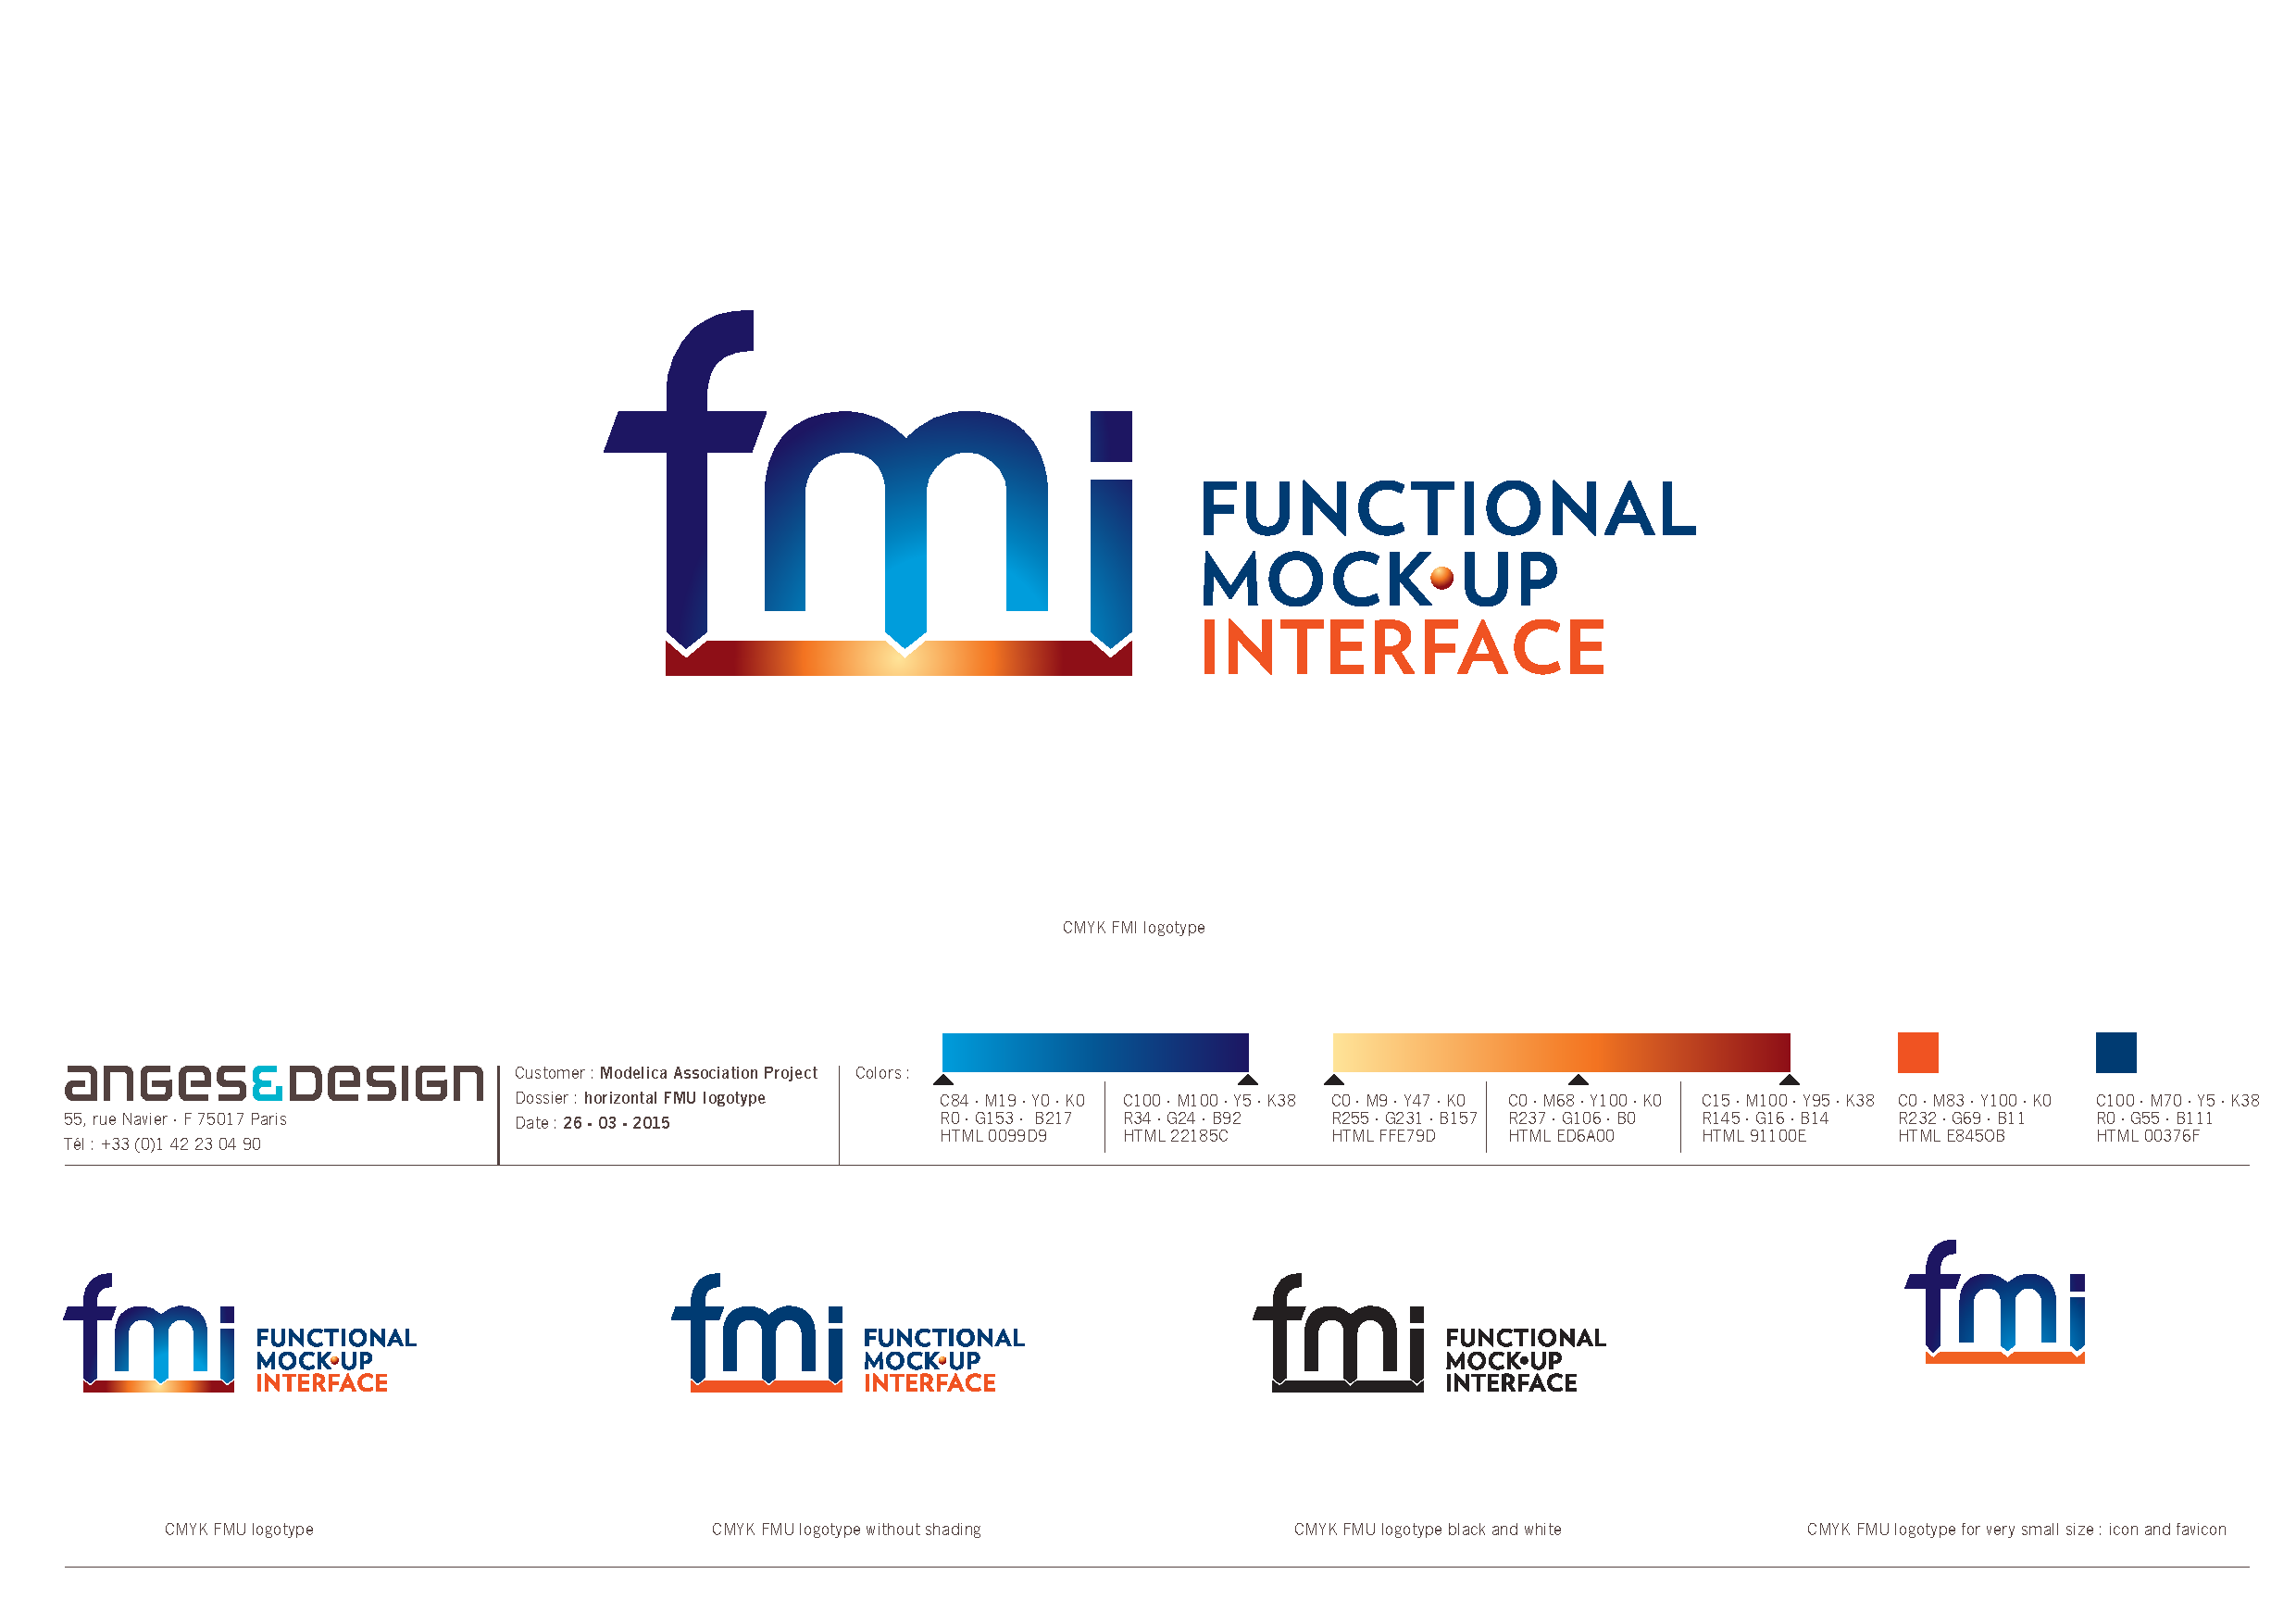
\includegraphics[height=1.85cm, clip=true, trim=10cm 16cm 10cm 5cm] {./figure/logotype_FMI_horizontal}}
  \vfilll
  \item A \alert{functional mock-up unit (FMU)} is a black box following the standard.
  % \tikzsetnextfilename{fmu}
  % \item PyFMI\footnote{\color{gray}\url{http://www.jmodelica.org/page/4924}} est un \alert{module \python} pour l'échange de modèle.
  \end{itemize}
  \vfilll
    \tikzexternaldisable{}
  \makebox[0.9\textwidth][c]%
  {%
    \centering
    \begin{tikzpicture}
      % \node[cellule]
      \coordinate (origin) at (0,0);
      \pic[file style, "XML", xshift=5mm] (xml) at (origin) {file icon};
      \foreach \x in {0,1,...,4}
      \path ([xshift=20mm, yshift=1mm] origin)++($\x*(2mm, -.5mm)$) node (fichier C \x) {X};

      \foreach \x in {0,1,...,4}
      \pic[file style, "C"] at (fichier C \x) {file icon};

      \node[cellule, fit=(origin) (fichier C 4) (xml-top), inner sep=2mm] (fmu) {};
      \node[etiquette, yshift=1mm, xshift=3mm] at (fmu.north west) {FMU};
    \end{tikzpicture}}
\fakefootnote{\color{gray}\url{https://www.fmi-standard.org/}}
\end{frame}

\section{\otfmi}

\begin{frame}{\otfmi: integrating \fmi{} support into \openturns}
  \begin{itemize}
  \item The new open source module \otfmi{} allows transparent use of \fmu{} with \openturns{} methods.
    \vfill
  \item It provides high level classes derived from \textpython{ot.PythonFunction}:\\running an \fmu{} instead of a \lpython{} function only requires to \alert{change~a~single~code~line}!
  \end{itemize}
\vfill
  \makebox[\textwidth][c]{\centering%
\pythonfile{./python/instantiate.py}
}\end{frame}

\begin{frame}{Implementation overview}
\tikzexternaldisable{}

\newcommand{\nudge}{10mm}
\makebox[\textwidth][c]{\centering
  \begin{tikzpicture}
    \tikzset{layer/.style={gray},
      limit/.style={thick, dashed, layer},
      realm/.style={opacity=.2},
      new/.style={draw=red, text={red}},
    node distance=15mm}

    \pgfdeclarelayer{foreground}
    \pgfdeclarelayer{background}
    \pgfsetlayers{background,main,foreground}

    \node[cellule] (tool) at (0,0) {Modelica tool GUI};

    \coordinate[below=of tool,  xshift=\nudge] (mos);
    \coordinate[below=of tool, xshift=-10mm] (zmo);
    \pic[file style, "script.mos", gray] at (mos)  {file icon};
    \node[cellule, below=18mm of mos] (compiler) {compiler};

    \coordinate (mo) at (zmo|-compiler);
    \pic[file style, "model.mo"] at (mo) {file icon};

    \coordinate[below=20mm of mo] (C);
    \pic[file style, "compiled C"] at (C)  {file icon};
    \coordinate[xshift=15mm] (fmu) at (C-|compiler);
    \pic[file style, "FMU"] at (fmu)  {file icon};


    \node[cellule, xshift=14mm, yshift=0mm] (fmi lib) at (fmu|-compiler) {FMI lib};
    \node[cellule, above right=5mm and 3mm of fmi lib] (pyfmi)  {\module{PyFMI}};
    \node[cellule, above left=5mm of pyfmi, new] (otfmi)  {\otfmi};
    \node[cellule, above right=5mm of pyfmi] (openturns)  {\openturns};
    \node[cellule, xshift=0mm, yshift=0mm] (openturns gui) at (pyfmi|-tool) {\openturns{} GUI};

    \begin{pgfonlayer}{background}
      \node[realm, above left=4mm and -10mm of compiler] {
\includegraphics[height=15mm] {./figure/logo_modelica}};
      \node[realm, above left=4mm and -10mm of fmu] {
\includegraphics[clip=true, height=15mm, trim=0mm 0mm 40mm 0mm] {./figure/logo_fmi}};
      \node[realm, above left=-4mm and 2mm of openturns] {
\includegraphics[height=15mm] {./figure/logo_openturns}};
      \node[realm, below left=-0mm and -4mm of pyfmi.north] {
\includegraphics[height=12mm] {./figure/logo_python}};

      % \node[realm] at (fmu) {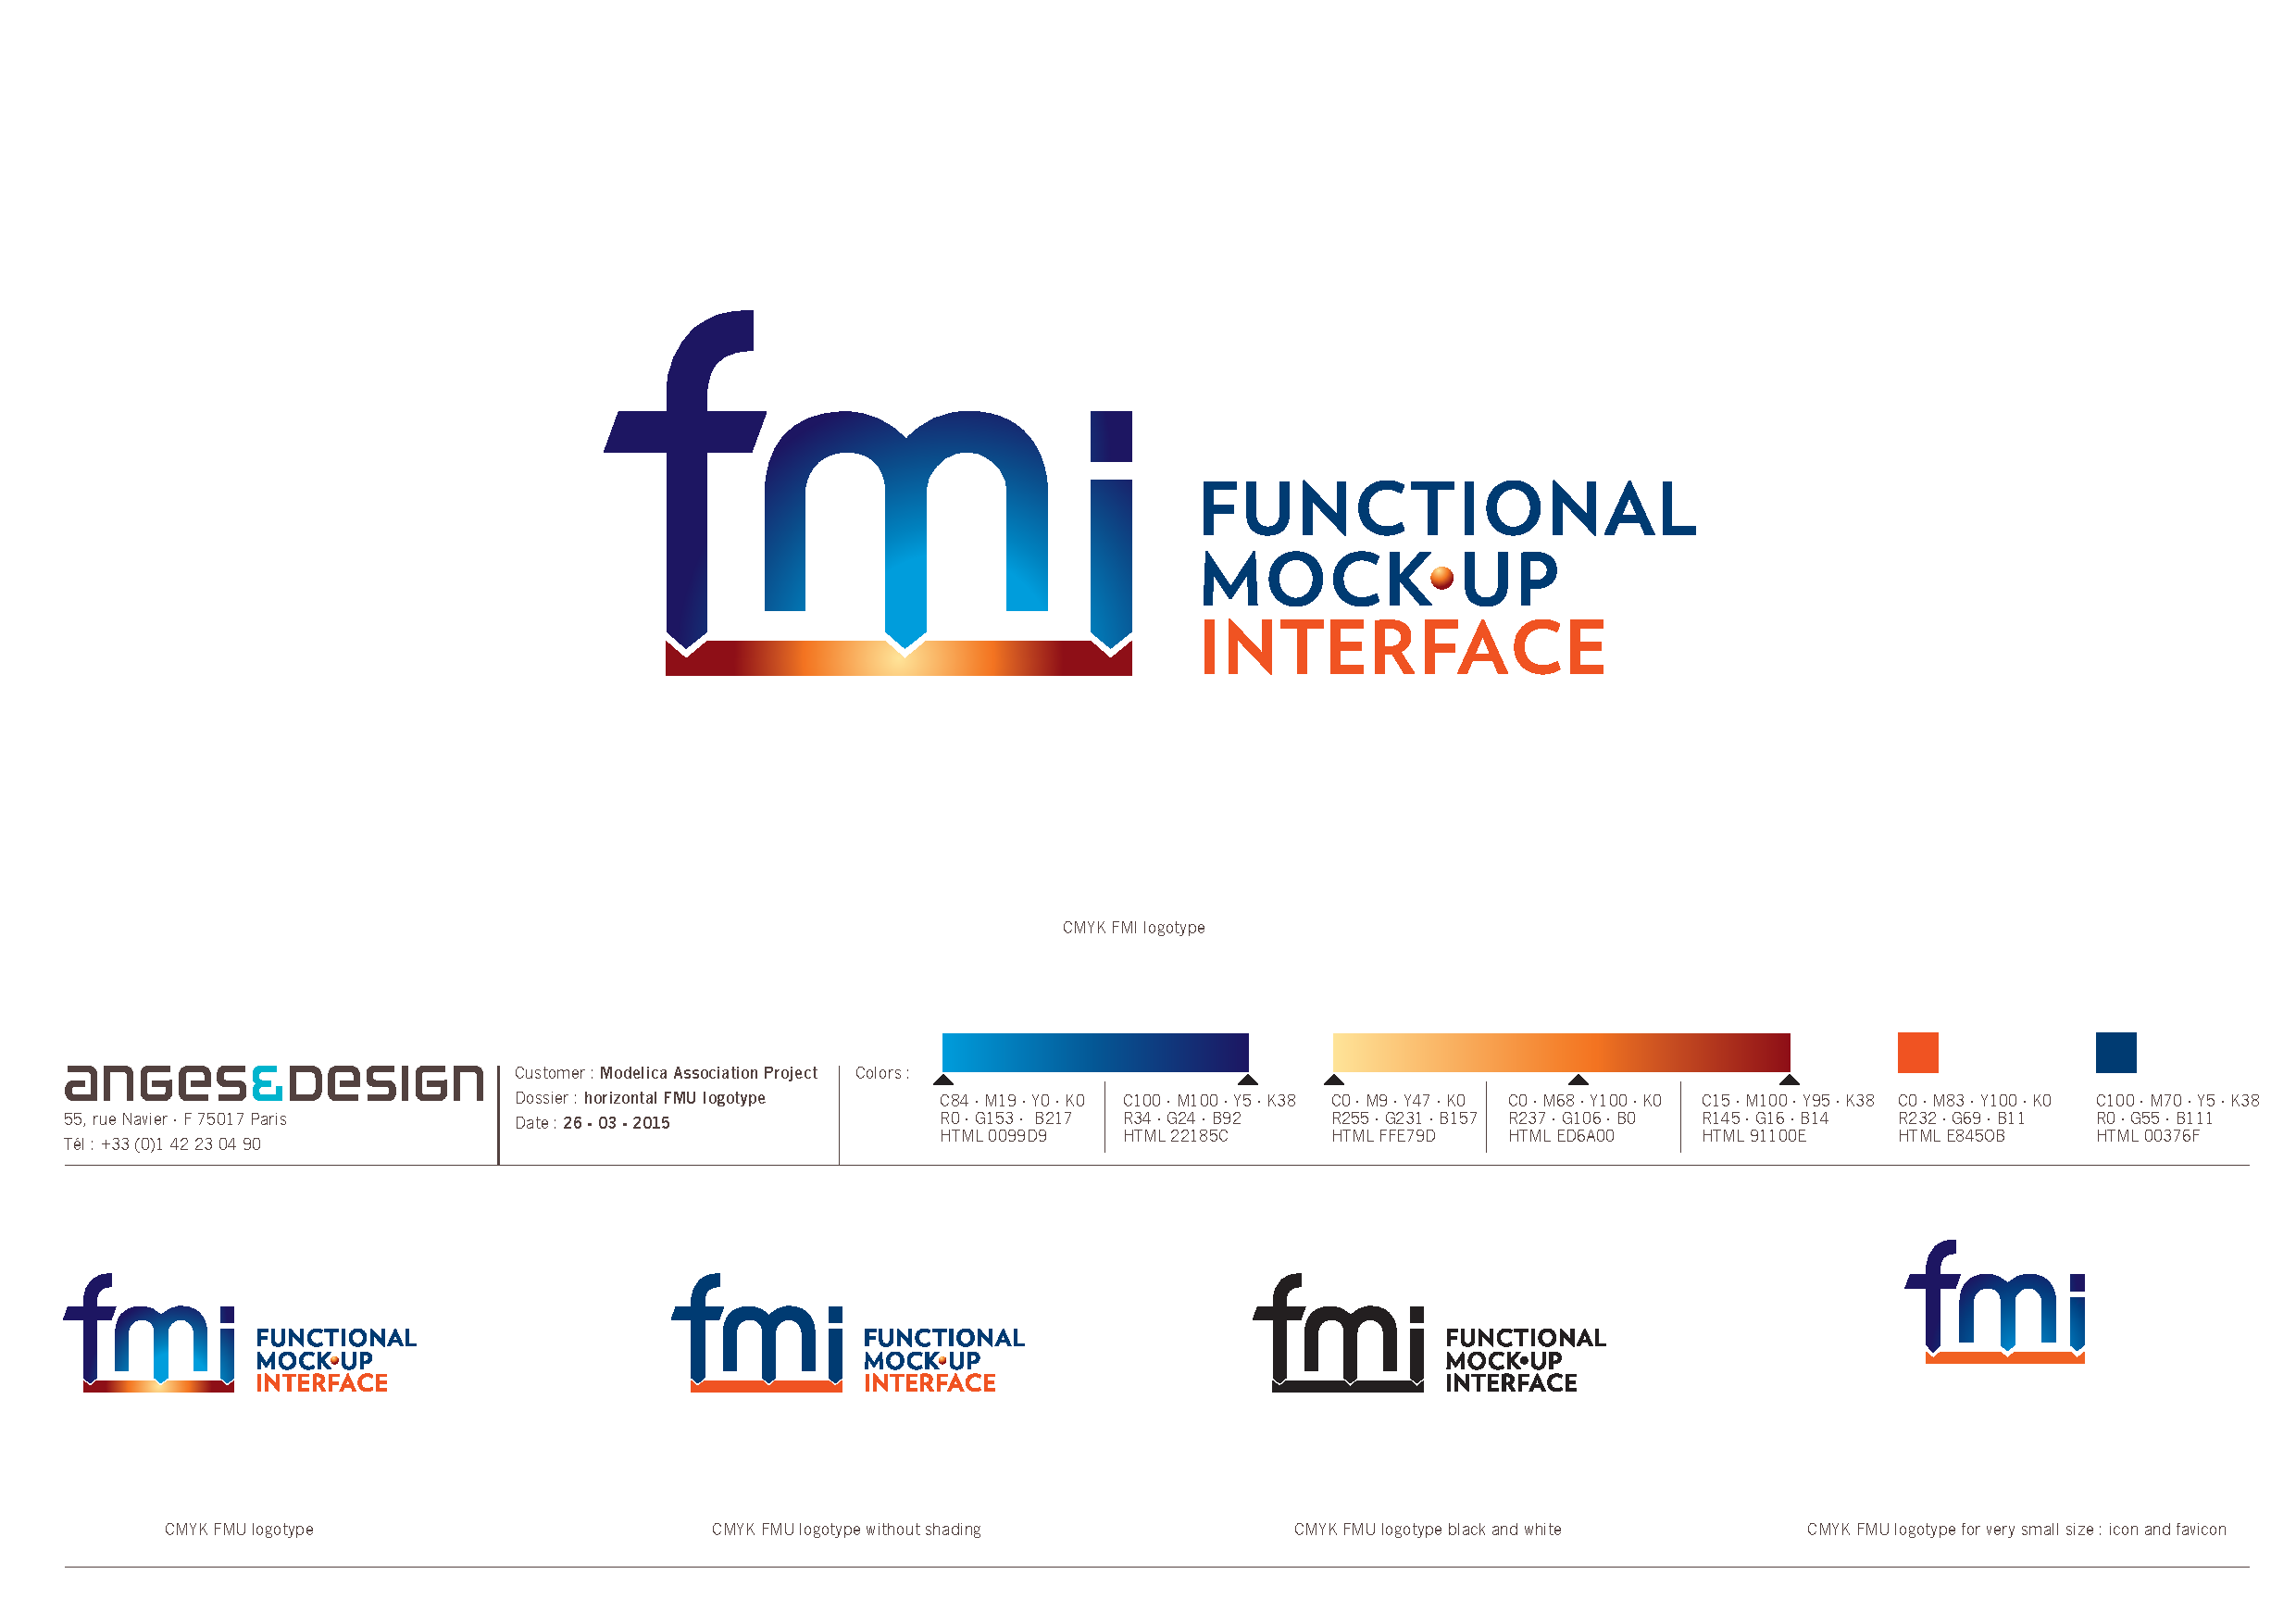
\includegraphics[height=10mm, clip=true, trim=10cm 16cm 10cm 5cm] {./figure/logotype_FMI_horizontal}};


      \coordinate (west) at (tool.west);
      \coordinate (east) at (openturns.east);
      \coordinate (y gui) at ([yshift=-2mm] tool.south);
      \coordinate (y code) at ([yshift=3mm] fmi lib.north);
      \draw[limit]  ([xshift=-2mm]west|-y gui) -- ([xshift=2mm]east|-y gui) coordinate (limit gui);
      \draw[limit]  ([xshift=-2mm]west|-y code) -- (limit gui|-y code) coordinate (limit code);

      \node[layer, above left=2mm and -3mm of limit gui] {Graphical};
      \node[layer, above left=2mm and -3mm of limit code] {Code};
      \node[layer, left=-3mm] at (fmu.south-|limit gui) {Compiled};


      \draw[link] ([xshift=1mm]tool.south) to[in=90, out=-90] (compiler);
      \draw[link, shorten >=6mm] ([xshift=-1mm]tool.south) to [in=90, out=-90] (mo);
      \draw[link] (mo) to (compiler);

      \draw[link, shorten >=6mm] ([xshift=-1mm]compiler.south) to[in=45, out=-90] (C);
      \draw[link, shorten >=7mm] ([xshift=2mm]compiler) to[in=140, out=-90] (fmu);

      \draw[link] (fmu) to[out=0,in=-90] (fmi lib);
      \draw[link] (fmi lib) to [out=0,in=-90] (pyfmi);
      \draw[link, new] (pyfmi) to [out=170,in=-90] (otfmi)
                          to[out=680, in=180] ([yshift=-2mm]openturns.west);
      \draw[link, new] (openturns) to [out=180,in=-90] (openturns gui);
     \end{pgfonlayer}

\end{tikzpicture}
}\end{frame}

\section{\otfmi{} grahical interface}

\begin{frame}{\otfmi{} grahical interface}
Motivations
\begin{itemize}
\item Provide access to \openturns{}' methods for \lmodelica{} users unfamiliar~with~\lpython{}
\item Considerably ease simple studies
\end{itemize}
\vfill
Issues
\begin{itemize}
\item \lmodelica{} models often define \alert{hundreds or thousands of variables}
\end{itemize}
\end{frame}

\begin{frame}{\otfmi{} grahical interface, \fmu{} overview}
\makebox[\textwidth][c]{\centering%
  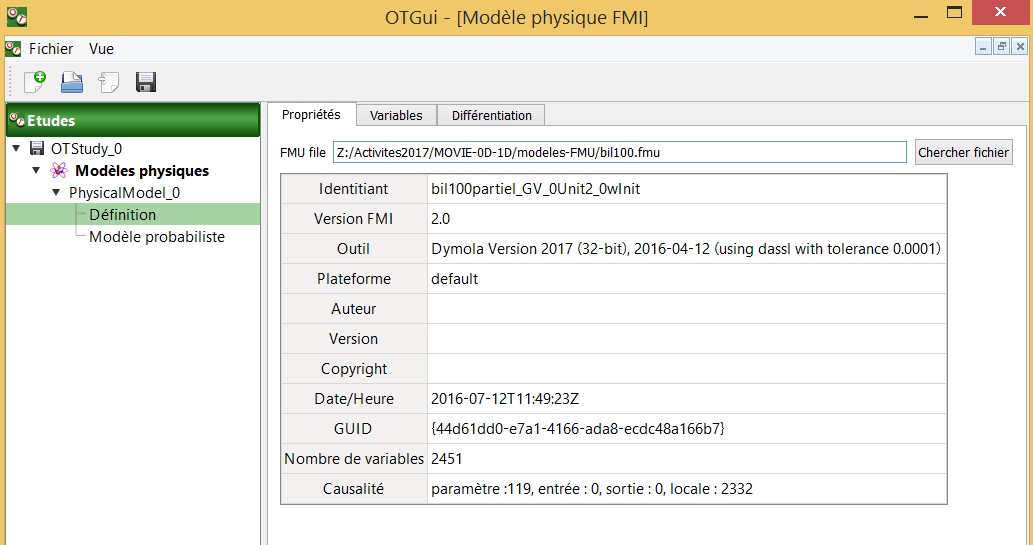
\includegraphics[height=.6\textheight]{./figure/bil100-resume}
}\end{frame}

\begin{frame}{\otfmi{} grahical interface, picking inputs and outputs}
\makebox[\textwidth][c]{\centering%
  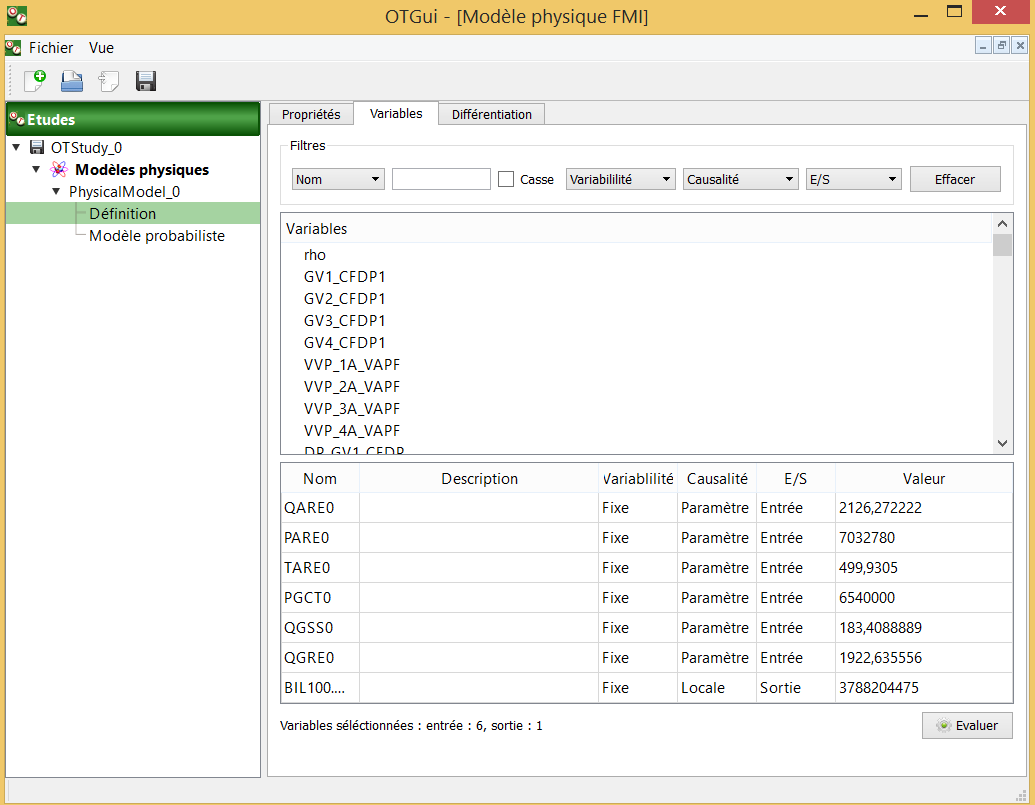
\includegraphics[height=.6\textheight]{./figure/bil100-variables}
}\end{frame}

\section*{}

\begin{frame}{Perspectives}
  \begin{itemize}
  \item Most 0D/1D system model are dynamical.\\
    We need methods for sensitivity analysis and emulation of model with \alert{time series inputs or outputs}.
    \vfill
  \item EDF is interested into \alert{data assimilation} with its \lmodelica{} models.
    \vfill
  \item What are the opportunities of \alert{extending the \lmodelica{} language} to support stochastic description of variables?
  % \item Information about the stochastic
  \end{itemize}
\end{frame}

\section*{}
\pagestyle{empty}
\begin{frame}
\vfill
\vfill
\hfill{}\huge\structure{Thank you for your attention.}

\end{frame}

\end{document}

%%% Local Variables:
%%% mode: latex
%%% TeX-master: t
%%% eval: (ispell-change-dictionary "british")
%%% End:
